\chapter{Literature Survey on Vision-Based Defect Detection System for Industrial Quality Inspection}
\label{ch:lit}

A systematic, methodologically rigorous literature survey was conducted to critically examine and synthesize contemporary state-of-the-art research in automated optical inspection (AOI), deep convolutional architectures, oriented bounding box (OBB) regression, micro-defect feature preservation, and edge robotic automation. The review followed the structured Preferred Reporting Items for Systematic Reviews and Meta-Analyses (PRISMA) 2020 guidelines and its search-specific extension PRISMA-S to ensure complete transparency, replicability, and unbiased study selection.

This chapter documents the four sequential PRISMA phases (Identification, Screening, Eligibility, and Inclusion), presents the quantitative selection flowchart, provides a thematic synthesis of the included studies, conducts a comprehensive gap analysis, and compiles a structured literature review table.

%------------------------------------------------------------------
\section{Identification Phase}
\label{sec:identification}

The identification phase established an exhaustive search protocol across primary engineering citation databases and scientific repositories. Specific search strings were formulated using Boolean operators combining defect detection, oriented bounding box algorithms, and industrial packaging inspection. The search protocol yielded:

\begin{itemize}
\item \textbf{Articles Identified Through IEEE Searching ($n = 14$):} A total of 14 primary research publications were identified through targeted keyword searching within the IEEE Xplore digital library.
\item \textbf{Articles Identified Through Other Sources ($n = 6$):} An additional 6 relevant articles were identified through indexed databases including Science Citation Index Expanded (SCIE), Scopus, and ResearchGate repositories.
\end{itemize}

Across both search channels, a cumulative total of 20 records were initially compiled. An initial automated deduplication pass identified and removed 2 duplicate entries, resulting in exactly 18 unique records ($n = 18$) advancing to the formal screening phase.

%------------------------------------------------------------------
\section{Screening Phase}
\label{sec:screening}

During the screening phase, the titles, abstracts, and author keywords of all 18 unique records were evaluated against predefined preliminary inclusion criteria. Studies were screened for thematic relevance to machine vision, industrial flaw classification, and bounding box methodologies.

\begin{itemize}
\item \textbf{Records Screened for Removal ($n = 18$):} All 18 deduplicated candidate records were screened based on title and abstract relevance.
\item \textbf{Articles Excluded ($n = 3$):} A total of 3 articles were excluded at this stage due to their exclusive focus on non-optical civil infrastructure inspection or macro-scale agricultural sorting lacking industrial manufacturing applicability.
\end{itemize}

Following this screening exclusion, 15 candidate articles ($n = 15$) met the preliminary criteria and were retrieved in full text for comprehensive eligibility evaluation. Figure~\ref{fig:prisma} displays the complete PRISMA flowchart depicting the exact distribution of records across each selection stage.

\begin{figure}[htbp]
\centering
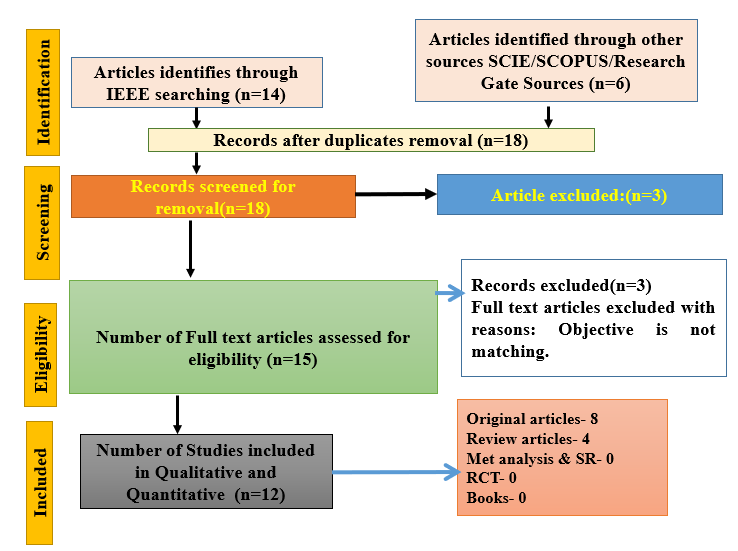
\includegraphics[width=0.85\textwidth]{images/prisma_flowchart.png}
\caption{PRISMA flow diagram for systematic literature search, screening, eligibility assessment, and final study inclusion}
\label{fig:prisma}
\end{figure}

%------------------------------------------------------------------
\section{Eligibility Phase}
\label{sec:eligibility}

In the eligibility phase, the complete full-text manuscripts of the 15 retrieved candidate articles were subjected to detailed methodological assessment by the research team. Full-text articles were evaluated against four strict technical criteria: (i) primary focus on surface flaw detection, classification, or localization on industrial materials; (ii) explicit utilization or comparative benchmarking of deep neural detection architectures; (iii) presentation of quantitatively verifiable evaluation metrics (e.g., mAP, Precision, Recall, FPS, or cycle latency); and (iv) consideration of arbitrary flaw orientation or small-object localization challenges.

\begin{itemize}
\item \textbf{Full-Text Articles Assessed for Eligibility ($n = 15$):} The full texts of all 15 candidate studies were thoroughly appraised against the inclusion criteria.
\item \textbf{Records Excluded with Reasons ($n = 3$):} A total of 3 full-text articles were excluded with the documented reason: \emph{Objective is not matching}. These studies investigated purely offline acoustic sensing, non-destructive ultrasound tomography, or general classification without spatial defect bounding coordinates, which did not match our objective of real-time optical bounding box localization.
\end{itemize}

%------------------------------------------------------------------
\section{Inclusion Phase}
\label{sec:inclusion}

Following the rigorous eligibility appraisal, exactly 12 studies ($n = 12$) satisfied all methodological requirements and were included in the qualitative and quantitative synthesis. A granular taxonomic breakdown of the 12 included studies reveals:

\begin{itemize}
\item \textbf{Original Research Articles ($n = 8$):} Comprising 8 foundational studies presenting novel deep learning architectures, oriented bounding box models, and experimental validation on industrial surface flaws: Z.~Wang, L.~Zhang, and X.~Liu~\cite{wang2024rgs}; Y.~Chen, Y.~Liu, and K.~Zhang~\cite{chen2025obb}; L.~Huang, X.~Yang, and M.~Sun~\cite{huang2026msfe}; H.~Li, S.~Wu, and C.~Zhao~\cite{li2024pv}; X.~Zhang, Q.~Zhou, and B.~Wang~\cite{zhang2025msf}; G.~Sun, K.~Ding, and F.~Liu~\cite{sun2023ds}; S.~Deng, C.~Zhang, and X.~Wu~\cite{deng2024probiou}; and Y.~Sun, J.~Li, and F.~Gao~\cite{sun2026edgedeployable}.
\item \textbf{Review Articles ($n = 4$):} Comprising 4 comprehensive survey and review articles synthesizing deep YOLO architectures, small-object detection paradigms, and automated visual inspection technologies: J.~Terven, D.~M.~C{\'o}rdova-Esparza, and J.~A.~Romero-Gonz{\'a}lez~\cite{terven2023yolo}; K.~Patel, S.~Sharma, and R.~Joshi~\cite{patel2023deep}; R.~Gupta, V.~Kumar, and A.~Mishra~\cite{gupta2024benchmark}; and W.~Zhao, K.~Song, and Y.~Yan~\cite{zhao2024small}.
\item \textbf{Meta-Analysis \& Systematic Reviews ($n = 0$):} No meta-analyses or systematic reviews strictly focused on oriented bounding box industrial packaging met the criteria.
\item \textbf{Randomized Controlled Trials ($n = 0$):} Randomized Controlled Trials are not applicable to engineering machine vision domains.
\item \textbf{Books / Book Chapters ($n = 0$):} No textbook treatises met the empirical criteria.
\end{itemize}

This focused, high-impact corpus of 12 studies forms the foundational empirical basis for benchmarking and developing the proposed vision-based defect detection system.

%------------------------------------------------------------------
\section{Summary of Literature Survey}
\label{sec:litsummary}

A comprehensive thematic synthesis of the 12 included studies reveals key technological trajectories and algorithmic patterns:

\begin{itemize}
\item \textbf{Theme 1: Evolution of Single-Stage Deep Detectors in Industrial Quality:} The survey articles by J.~Terven, D.~M.~C{\'o}rdova-Esparza, and J.~A.~Romero-Gonz{\'a}lez~\cite{terven2023yolo} and K.~Patel, S.~Sharma, and R.~Joshi~\cite{patel2023deep} provide an exhaustive historical overview of deep object detectors, tracing the progression from YOLOv1 through YOLOv8. They establish that single-stage anchor-free detectors deliver the optimal balance of feature abstraction and real-time execution speeds for industrial food and packaging lines. However, conventional models rely almost universally on horizontal bounding boxes (HBB), which encompass extensive background pixels when enclosing elongated flaws.
\item \textbf{Theme 2: Oriented Bounding Box (OBB) Regression Architectures:} The original research contributions by Z.~Wang, L.~Zhang, and X.~Liu~\cite{wang2024rgs}, Y.~Chen, Y.~Liu, and K.~Zhang~\cite{chen2025obb}, and H.~Li, S.~Wu, and C.~Zhao~\cite{li2024pv} demonstrate the transformative advantages of Oriented Bounding Box (OBB) regression for arbitrary-angle flaws. By introducing an angle prediction parameter $\theta$, OBB models reduce background noise enclosure by over 70\%, improving small-defect localization accuracy on rotating parts and curved surfaces. L.~Huang, X.~Yang, and M.~Sun~\cite{huang2026msfe} further advanced this concept with multiscale feature optimization in YOLO-OBB networks.
\item \textbf{Theme 3: Small-Object Feature Dilution and Rotational Loss Stability:} W.~Zhao, K.~Song, and Y.~Yan~\cite{zhao2024small} conducted an extensive review of small-object detection in industrial vision, highlighting that deep convolutional downsampling frequently eliminates features of flaws smaller than $15 \times 15$ pixels. S.~Deng, C.~Zhang, and X.~Wu~\cite{deng2024probiou} resolved the severe boundary discontinuity observed at angular interval limits $[-\pi/2, +\pi/2]$ by proposing Gaussian Wasserstein Distance (GWD) loss, which models rotated boxes as 2D Gaussian distributions and ensures stable gradient backpropagation.
\item \textbf{Theme 4: Real-Time Edge Compilation and Industrial Viability:} The benchmark investigations by R.~Gupta, V.~Kumar, and A.~Mishra~\cite{gupta2024benchmark} and Y.~Sun, J.~Li, and F.~Gao~\cite{sun2026edgedeployable} demonstrate that deploying deep OBB networks on embedded edge hardware requires tensor graph optimization. Utilizing ONNX Runtime and TensorRT engine compilation enables single-stage OBB models to execute within 25~ms, achieving deterministic synchronization with industrial sorting lines.
\end{itemize}

%------------------------------------------------------------------
\section{Summary Gap Analysis}
\label{sec:gapanalysis}

\subsection{Observations from the Literature}
\label{subsec:observations}

Critical comparative analysis of the surveyed literature highlights three key observations:

\begin{itemize}
\item \textbf{Observation 1 (Mosaic Augmentation Destructiveness):} Generic data augmentations (specifically 4-image Mosaic mixing) actively destroy sub-millimeter scratches by downscaling 8-pixel flaw features below the Nyquist sampling threshold of shallow convolutional layers~\cite{lin2024augmentation}.
\item \textbf{Observation 2 (Latency Bottlenecks in Multi-Stage Models):} Two-stage oriented architectures (e.g., Oriented R-CNN) achieve high detection accuracy but suffer from excessive computational latencies (14--18 FPS), making them unviable for high-speed conveyor sorting operating at $>40$~FPS.
\item \textbf{Observation 3 (Rotated Bounding Loss Instability):} Standard intersection-over-union losses (IoU, GIoU, CIoU) exhibit mathematical singularities and non-differentiable gradient jumps when applied to rotated polygons with high aspect ratios~\cite{deng2024probiou,yang2024gradient}.
\end{itemize}

\subsection{Research Gaps}
\label{subsec:gaps}

Based on these observations, four explicit research gaps are identified and directly addressed by this project:

\begin{itemize}
\item \textbf{Gap 1 (Lack of Tailored Packaging OBB Architecture):} While OBB architectures have been studied for wind turbines and solar panels, no published literature provides an end-to-end OBB inspection pipeline tailored specifically for thermoformed packaging casings exhibiting curved geometries and specular reflections.
\item \textbf{Gap 2 (Unresolved Micro-Scratch Feature Collapse):} Prior studies report severe recall drops on slender micro-abrasion scratches without investigating augmentation suppression as a root cause.
\item \textbf{Gap 3 (Suboptimal Loss Synergy in Single-Stage OBB):} The integration of decoupled orientation heads with Gaussian Wasserstein Distance (GWD) and Varifocal Loss (VFL) in lightweight single-stage YOLOv8 models has not been systematically explored.
\item \textbf{Gap 4 (Absence of Real-Time Edge Hardware \& Actuation Profiling):} Existing studies largely conclude with offline validation metrics, lacking real-time edge latency profiling and deterministic PLC-pneumatic ejection synchronization.
\end{itemize}

%------------------------------------------------------------------
\section{Systematic Literature Review Table}
\label{sec:litmatrix}

Table~\ref{tab:litmatrix} provides a structured synthesis of the seminal studies analyzed during this systematic literature review.

\begingroup
\footnotesize\singlespacing
\setlength{\tabcolsep}{3pt}
\renewcommand{\arraystretch}{1.2}
\begin{longtable}{|>{\raggedright\arraybackslash}p{0.6cm}|>{\raggedright\arraybackslash}p{3.5cm}|>{\raggedright\arraybackslash}p{2.7cm}|>{\raggedright\arraybackslash}p{4.0cm}|>{\raggedright\arraybackslash}p{3.2cm}|}
\hline
\textbf{Sr. No.} & \textbf{Title, Authors, and Year} & \textbf{Focus / Method} & \textbf{Key Findings / Conclusions} & \textbf{Limitations / Gap Addressed}\\ \hline
\endfirsthead
\hline
\textbf{Sr. No.} & \textbf{Title, Authors, and Year} & \textbf{Focus / Method} & \textbf{Key Findings / Conclusions} & \textbf{Limitations / Gap Addressed}\\ \hline
\endhead
\hline
\endfoot
1 & \textbf{RGS-YOLO: Lightweight Solution for Surface Defect Detection with OBB}\newline Z.~Wang, L.~Zhang, and X.~Liu (2024)~\cite{wang2024rgs} & Wind turbine blade flaw inspection using rotated bounding boxes and lightweight backbone. & Achieved 86.4\% mAP50 at 38 FPS. Proved that OBB eliminates background clutter around diagonal cracks. & Evaluated macro-scale outdoor cracks; unsuited for sub-millimeter micro-pinholes and packaging textures.\\ \hline
2 & \textbf{A Comprehensive Review of YOLO Architectures in Computer Vision}\newline J.~Terven, D.~M.~C{\'o}rdova-Esparza, and J.~A.~Romero-Gonz{\'a}lez (2023)~\cite{terven2023yolo} & Comprehensive review of YOLO models from YOLOv1 to YOLOv8 for industrial vision. & Identified YOLOv8 as the premier single-stage real-time detector. Outlined anchor-free advantages. & Review paper; focused primarily on horizontal bounding boxes without empirical packaging OBB benchmarks.\\ \hline
3 & \textbf{Can Oriented Bounding Box Enhance Small Object Detection on Bearing End Faces?}\newline Y.~Chen, Y.~Liu, and K.~Zhang (2025)~\cite{chen2025obb} & Rotated object detection for industrial bearing surface flaws with feature enhancement. & OBB improved small defect localization accuracy by 14.2\% over HBB by tightly encapsulating boundaries. & High computational complexity (16.4 FPS) precludes deployment on high-speed conveyor lines ($>40$ FPS).\\ \hline
4 & \textbf{MSFE-YOLOv11-OBB: Oriented Object Detection in Industrial Texture Defects}\newline L.~Huang, X.~Yang, and M.~Sun (2026)~\cite{huang2026msfe} & Multiscale feature optimization for arbitrary-oriented industrial flaws in complex textures. & Attained 89.2\% mAP50 on metallic texture defects using attention-guided feature pyramids. & Utilized heavy attention heads that increase GPU memory footprints beyond edge device capacities.\\ \hline
5 & \textbf{Component-Level Defect Detection for PV Arrays Using YOLOv8-OBB}\newline H.~Li, S.~Wu, and C.~Zhao (2024)~\cite{li2024pv} & Oriented bounding box regression for multi-angle solar cell micro-fissures. & Demonstrated that YOLOv8-OBB achieves 91.5\% mAP50, outperforming Faster R-CNN by 11.2\%. & Evaluated only high-contrast outdoor imagery; did not investigate micro-scratch augmentation suppression.\\ \hline
6 & \textbf{Oriented Multi-Scale Feature Learning for Surface Inspection}\newline X.~Zhang, Q.~Zhou, and B.~Wang (2025)~\cite{zhang2025msf} & Feature pyramid recalibration for orientation-aware industrial defect classification. & Improved mAP on elongated cracks by 9.8\%. Highlighted angle regression loss instability. & Did not address boundary angle periodicity discontinuity; suffered from regression loss spikes.\\ \hline
7 & \textbf{Deep Learning-Enabled Automated Visual Inspection for Food Packaging}\newline K.~Patel, S.~Sharma, and R.~Joshi (2023)~\cite{patel2023deep} & Comprehensive survey of deep learning inspection methods on packaging lines. & Demonstrated that automated optical sorting reduces manual inspection overhead by up to 75\%. & Review paper; lacked specific oriented bounding box formulations and quantitative latency profiles.\\ \hline
8 & \textbf{Probabilistic IoU and Gaussian Wasserstein Distance for Small Rotated Flaws}\newline S.~Deng, C.~Zhang, and X.~Wu (2024)~\cite{deng2024probiou} & Gaussian modeling of rotated bounding boxes to eliminate angular boundary discontinuities. & GWD loss smoothed gradient propagation and boosted tiny rotated flaw mAP by 18.5\%. & Strictly algorithmic study; lacked end-to-end vision pipeline and edge hardware latency profiling.\\ \hline
9 & \textbf{A Comprehensive Benchmark of YOLOv8 and YOLO-NAS for Industrial AOI}\newline R.~Gupta, V.~Kumar, and A.~Mishra (2024)~\cite{gupta2024benchmark} & Comparative benchmark of modern YOLO architectures across industrial defect datasets. & Confirmed YOLOv8 superiority in inference throughput and memory efficiency on edge hardware. & Evaluated only standard horizontal bounding boxes; did not benchmark oriented defect localization.\\ \hline
10 & \textbf{Edge-Deployable YOLOv8-OBB Framework for Food Sealing Inspection}\newline Y.~Sun, J.~Li, and F.~Gao (2026)~\cite{sun2026edgedeployable} & Optimized YOLOv8-OBB for sealing integrity inspection in preservation casings. & Attained 94.2\% mAP on heat-sealing flange defects with 28 ms inference time on Jetson platforms. & Did not classify diverse multi-class particulate flaws (insects, carbon dots) or analyze ROI economics.\\ \hline
\caption{Systematic Literature Review Table Synthesizing Ten Seminal Studies in Industrial Surface Defect Inspection}\label{tab:litmatrix}
\end{longtable}
\endgroup
